% ---------------------------------------------------------------------------
% ---------------------------------------------------------------------------
% Modelo LaTex para preparação do documento final de Monografia TCC
% O modelo está em conformidade com ABNT NBR
% Faculdade do Piaui
% ---------------------------------------------------------------------------
% ---------------------------------------------------------------------------

\documentclass[
	% -- opções da classe memoir --
	12pt,					% tamanho da fonte
	openright,				% capítulos começam em pág ímpar (insere página vazia caso preciso)
	%twoside,					% para impressão em verso e anverso. Oposto a oneside
	a4paper,					% tamanho do papel. 
	% -- opções da classe abntex2 --
	%chapter=TITLE,			% títulos de capítulos convertidos em letras maiúsculas
	%section=TITLE,			% títulos de seções convertidos em letras maiúsculas
	%subsection=TITLE,		% títulos de subseções convertidos em letras maiúsculas
	%subsubsection=TITLE,	% títulos de subsubseções convertidos em letras maiúsculas
	% -- opções do pacote babel --
	english,					% idioma adicional para hifenização
	%french,					% idioma adicional para hifenização
	%spanish,				% idioma adicional para hifenização
	brazil					% o último idioma é o principal do documento
	]{abntex2}

% ---------------------
% Pacotes OBRIGATÓRIOS
% ---------------------
\usepackage{float}
\floatstyle{boxed} 
\restylefloat{figure}
\usepackage{lmodern}				% Usa a fonte Latin Modern			
\usepackage[T1]{fontenc}			% Selecao de codigos de fonte.
\usepackage[utf8]{inputenc}		% Codificacao do documento (conversão automática dos acentos)
\usepackage{lastpage}			% Usado pela Ficha catalográfica
\usepackage{indentfirst}			% Indenta o primeiro parágrafo de cada seção.
\usepackage{color}				% Controle das cores
\usepackage{graphicx,graphicx}	% Inclusão de gráficos
\usepackage{epsfig,subfig}		% Inclusão de figuras
\usepackage{microtype} 			% Melhorias de justificação
% ---------------------
		
% ---------------------
% Pacotes ADICIONAIS
% ---------------------
\usepackage{lipsum}						% Geração de dummy text
\usepackage{amsmath,amssymb,mathrsfs}	% Comandos matemáticos avançados 
\usepackage{setspace}  					% Para permitir espaçamento simples, 1 1/2 e duplo
\usepackage{verbatim}					% Para poder usar o ambiente "comment"
\usepackage{tabularx} 					% Para poder ter tabelas com colunas de largura auto-ajustável
\usepackage{afterpage} 					% Para executar um comando depois do fim da página corrente
\usepackage{url} 						% Para formatar URLs (endereços da Web)
% ---------------------

% ---------------------
% Pacotes de CITAÇÕES
% ---------------------
\usepackage[brazilian,hyperpageref]{backref}	% Paginas com as citações na bibl
\usepackage[alf]{abntex2cite}				% Citações padrão ABNT (alfa)
%\usepackage[num]{abntex2cite}				% Citações padrão ABNT (numericas)
% ---------------------

% Configurações de CITAÇÕES para abntex2
% --- 
% CONFIGURAÇÕES DE PACOTES
% --- 

% ---
% Configurações do pacote backref
% Usado sem a opção hyperpageref de backref
\renewcommand{\backrefpagesname}{Citado na(s) página(s):~}
% Texto padrão antes do número das páginas
\renewcommand{\backref}{}
% Define os textos da citação
\renewcommand*{\backrefalt}[4]{
	\ifcase #1 %
		Nenhuma citação no texto.%
	\or
		Citado na página #2.%
	\else
		Citado #1 vezes nas páginas #2.%
	\fi}%
% ---

% Inclusão de dados para CAPA e FOLHA DE ROSTO (título, autor, orientador, etc.)
% ---
% Informações de dados para CAPA e FOLHA DE ROSTO
% ---
\titulo{Desenvolvimento de um sistema web para controle de veículos e acesso aos estacionamentos dos campi do IFRN}
\autor{José Victor Gomes de França}
\local{Natal-RN}
\data{Novembro de 2019}
\orientador{Prof. Rafael Fernandes de Queiroz}
%\coorientador{Fulano Coorientador}
\instituicao{%
  Instituto Federal de Educação, Ciência e Tecnologia Rio Grande do Norte - IFRN}
\tipotrabalho{Trabalho de Conclusão de Curso (TCC)}
% O preambulo deve conter o tipo do trabalho, o objetivo,
% o nome da instituição e a área de concentração
\preambulo{\textbf{Trabalho de Conclusão de Curso} Monografia apresentada ao Instituto Federal de Educação, Ciência e Tecnologia Rio Grande do Norte (IFRN),  como pré-requisito para a obtenção do título de Técnico em Informática para Internet.}
% ---

% Inclui Configurações de aparência do PDF Final
%  Configurações de aparência do PDF final
% NÃO ALTERAR!!!

% alterando o aspecto da cor azul
\definecolor{blue}{RGB}{41,5,195}

% informações do PDF
\makeatletter
\hypersetup{
     	%pagebackref=true,
		pdftitle={\@title}, 
		pdfauthor={\@author},
    		pdfsubject={\imprimirpreambulo},
	    pdfcreator={LaTeX with abnTeX2},
		pdfkeywords={abnt}{latex}{abntex}{abntex2}{trabalho acadêmico}, 
		colorlinks=true,       		% false: boxed links; true: colored links
    		linkcolor=blue,          	% color of internal links
    		citecolor=blue,        		% color of links to bibliography
    		filecolor=magenta,      		% color of file links
		urlcolor=blue,
		bookmarksdepth=4
} 
\makeatother
% --- 

% O tamanho da identação do parágrafo é dado por:
\setlength{\parindent}{1.3cm}

% Controle do espaçamento entre um parágrafo e outro:
\setlength{\parskip}{0.2cm}  % tente também \onelineskip

% ---------------------
% Compila o indice
% ---------------------
\makeindex
% ---------------------

%%%%%%%%%%%%%%%%%%%%%%%%%%%
%%  INICIO DO DOCUMENTO  %%
%%%%%%%%%%%%%%%%%%%%%%%%%%%
\begin{document}

% Retira espaço extra obsoleto entre as frases.
\frenchspacing

% ----------------------------------------------------------
% ELEMENTOS PRÉ-TEXTUAIS (Capa, Resumo, Abstract, etc.)
% ----------------------------------------------------------
\pretextual

% Capa
% ---
% Impressão da Capa
% ---
  \begin{capa}%
    \begin{figure}[h!]%
        \centering%
        
\includegraphics[scale=0.5]{figs/download.png}%
      \end{figure}%
    \center
	\ABNTEXchapterfont\large{Instituto Federal de Educação, Ciência e Tecnologia Rio Grande do Norte\\Curso Técnico em Informática para Internet}
	%\vspace{1.5cm}

    \vfill
    \ABNTEXchapterfont\bfseries\LARGE\imprimirtitulo
    \vfill

	%\vfill
	\ABNTEXchapterfont\large\imprimirautor
	\vfill
%
    \large\imprimirlocal, \large\imprimirdata

    \vspace*{1cm}
  \end{capa}
% ---

% Folha de rosto (o * indica que haverá a ficha bibliográfica)
\imprimirfolhaderosto*

% Imprimir Ficha Catalografica
%% ---
% Ficha Catalográfica
% ---
% Isto é um exemplo de Ficha Catalográfica, ou ``Dados internacionais de
% catalogação-na-publicação''. Você pode utilizar este modelo como referência. 
% Porém, provavelmente a biblioteca da sua universidade lhe fornecerá um PDF
% com a ficha catalográfica definitiva após a defesa do trabalho. Quando estiver
% com o documento, salve-o como PDF no diretório do seu projeto e substitua todo
% o conteúdo de implementação deste arquivo pelo comando abaixo:
%
% \begin{fichacatalografica}
%     \includepdf{fig_ficha_catalografica.pdf}
% \end{fichacatalografica}
\begin{fichacatalografica}
	\vspace*{\fill}					% Posição vertical
	\hrule							% Linha horizontal
	\begin{center}					% Minipage Centralizado
	\begin{minipage}[c]{12.5cm}		% Largura
	
	\imprimirautor
	
	\hspace{0.5cm} \imprimirtitulo  / \imprimirautor. --
	\imprimirlocal, \imprimirdata-
	
	\hspace{0.5cm} \pageref{LastPage} p. : il. (algumas color.) ; 30 cm.\\
	
	\hspace{0.5cm} \imprimirorientadorRotulo~\imprimirorientador\\
	
	\hspace{0.5cm}
	\parbox[t]{\textwidth}{\imprimirtipotrabalho~--~\imprimirinstituicao,
	\imprimirdata.}\\
	
	\hspace{0.5cm}
		1. Palavra-chave1.
		2. Palavra-chave2.
		I. Orientador.
		II. Universidade xxx.
		III. Faculdade de xxx.
		IV. Título\\ 			
	
	\hspace{8.75cm} CDU 02:141:005.7\\
	
	\end{minipage}
	\end{center}
	\hrule
\end{fichacatalografica}
% ---

% Inserir Folha de Aprovação
% ---
% Assinaturas
% ---
% Isto é um exemplo de Folha de aprovação, elemento obrigatório da NBR
% 14724/2011 (seção 4.2.1.3). Você pode utilizar este modelo até a aprovação
% do trabalho. Após isso, substitua todo o conteúdo deste arquivo por uma
% imagem da página assinada pela banca com o comando abaixo:
%
% \includepdf{folhadeaprovacao_final.pdf}
%
\begin{folhadeaprovacao}

  \begin{center}
    {\ABNTEXchapterfont\large\imprimirautor}

    \vspace*{\fill}\vspace*{\fill}
    \begin{center}
      \ABNTEXchapterfont\bfseries\Large\imprimirtitulo
    \end{center}
    \vspace*{\fill}
    
    \hspace{.45\textwidth}
    \begin{minipage}{.5\textwidth}
        \imprimirpreambulo
    \end{minipage}%
    \vspace*{\fill}
   \end{center}
        
   Trabalho aprovado. \imprimirlocal, 01 de janeiro de 2014:

   \assinatura{\textbf{\imprimirorientador} \\ Orientador} 
   %\assinatura{\textbf{\imprimircoorientador} \\ Co-Orientador} 
   \assinatura{\textbf{Professor} \\ Convidado 1}
   \assinatura{\textbf{Professor} \\ Convidado 2}
   \assinatura{\textbf{Professor} \\ Convidado 3}
      
   \begin{center}
    \vspace*{0.5cm}
    {\large\imprimirlocal}
    \par
    {\large\imprimirdata}
    \vspace*{1cm}
  \end{center}
  
\end{folhadeaprovacao}
% ---

% Dedicatória
% ---
% Dedicatória
% ---
\begin{dedicatoria}
   \vspace*{\fill}
   \centering
   \noindent
   \textit{ Dedico esse trabalho aos meus queridos pais, minha triunfante e amada Mãe, Paula Frassinete Gomes França, e meu batalhador pai, José Vital de França. A eles dedico todo meu reconhecimento, gratidão e amor. Igualmente dedico esse trabalho as minhas igualmente amadas irmâs , Maria José Gomes de França, Ana Maria Gomes de França e Maria das Dores Gomes de França por todo apoio oferecido ao longo de minha vida. Desejo poder ter sido merecedor do esforço dedicado por vocês em todos os aspectos, especialmente quanto à minha formação. Também dedico este trabalho ao Leonardo Maximino Bernardo pelo companheirismo e felicidade proporcionados.} \vspace*{\fill}
\end{dedicatoria}
% ---

% Agradecimentos
% ---
% Agradecimentos
% ---
\begin{agradecimentos}

%Agradeço a Deus.

%Agradeço aos meus pais, XXXXX e YYYYY, por ...

%Aos meus irmãos, por.....

%Agradeço ao meu orientador, XXXXXXXXX, por todos os conselhos, pela paciência e ajuda nesse período.

%Aos meus amigos ...

%Aos professores ...

%À XXXXXX pelo apoio financeiro para realização deste trabalho de pesquisa.

Ao longo destes dois anos de estudo que resultaram neste trabalho de conclusão de curso, pessoas e
instituições me ajudaram, ensinando e apoiando. Agora que alcanço meus
objetivos, não poderia deixar de reconhecê-las.

Começo por agradecer a minha adorável e digníssima mãe, pilar seguro, colo de amor incondicional, Paula Frassinete Gomes França e ao meu amado e dedicado pai, José Vital de França. Desejo que esta minha conquista sirva de algum modo, se possível, como exemplo para minhas irmãs e irmãos.

Agradeço ao meu orientador, Prof. Rafael Fernandes de Queiroz, por ser meu guia nesta árdua tarefa de desenvolver esse sistema.

 

Meu reconhecimento aos professores, colegas e funcionários do curso de informática para internet EaD do IFRN.



\end{agradecimentos}
%% ---

% Epígrafe
% ---
% Epígrafe
% ---
\begin{epigrafe}
    \vspace*{\fill}
	\begin{flushright}
		\textit{``O que não provoca minha morte faz com que eu fique mais forte.''\\
		          (Friedrich Nietzsche)\\
	         % “Talvez não tenha conseguido fazer o melhor, mas lutei para que o melhor fosse feito. Não sou o que deveria ser, mas Graças a Deus, não sou o que era antes”. (Marthin Luther King)\\
          %``Ninguém é tão grande que não possa aprender, nem tão pequeno que não possa ensinar”.
          %
          %(Esopo)\\
      %``A inteligência é a insolência educada”.
      %(Aristóteles)
  }
	\end{flushright}
\end{epigrafe}
% ---

% Resumo e Abstract
% ---
% RESUMOS
% ---

% RESUMO em português
\setlength{\absparsep}{18pt} % ajusta o espaçamento dos parágrafos do resumo
\begin{resumo}
\emph{(Em construção:)}\,Tendo em vista que a quantidade de vagas no estacionamento do IFRN é limitado e a quantidade de veículos ocupantes está aumentando gradativamente, é necessário controlar os veículos que realmente devem ter acesso ao estacionamento do IFRN, tais como aqueles pertencentes a servidores do instituto. Além da quantidade, o processo para cadastro de um veículo é bastante burocrático, exigindo a comunicação entre várias pessoas (Diretor, Departamento de Segurança, etc.) para autorizar o cadastro do veículo, dificultando a aquisição do adesivo que identifica um veículo autorizado. O sistema deve ser desenvolvido utilizando o framework Ruby On Rails e banco de dados PostgreSQL, utilizando conhecimentos de diversas disciplinas do curso (APOO, PDSI, Banco de Dados, e outras).

 \textbf{Palavras-chaves}: latex. abntex. editoração de texto.
\end{resumo}

% ABSTRACT in english
\begin{resumo}[Abstract]
 \begin{otherlanguage*}{english}
   Given that the number of IFRN parking spaces is limited and the number of occupant vehicles is gradually increasing, it is necessary to control the vehicles that really should have access to the IFRN parking, such as those belonging to IFRN servants. In addition to the amount, the process for registering a vehicle is quite bureaucratic, requiring communication between several people (Director, Security Department, etc.) to authorize the registration of the vehicle, making it difficult to purchase the sticker that identifies an authorized vehicle. The system should be developed using the Ruby On Rails framework and PostgreSQL database, using knowledge of several course subjects (APOO, PDSI, Database, and others).

   \vspace{\onelineskip}
 
   \noindent 
   \textbf{Keywords}: latex. abntex. text editoration.
 \end{otherlanguage*}
\end{resumo}

% Lista de ilustrações
\pdfbookmark[0]{\listfigurename}{lof}
\listoffigures*
\cleardoublepage

% Lista de tabelas
\pdfbookmark[0]{\listtablename}{lot}
\listoftables*
\cleardoublepage

% Lista de abreviaturas e siglas
\begin{siglas}
  \item[ABNT] Associação Brasileira de Normas Técnicas
  \item[abnTeX] ABsurdas Normas para TeX
\end{siglas}

% Lista de símbolos
\begin{simbolos}
  \item[$ \Gamma $] Letra grega Gama
  \item[$ \Lambda $] Lambda
  \item[$ \zeta $] Letra grega minúscula zeta
  \item[$ \in $] Pertence
\end{simbolos}

% Inserir o SUMÁRIO
\pdfbookmark[0]{\contentsname}{toc}
\tableofcontents*
\cleardoublepage

% ----------------------------------------------------------
% ELEMENTOS TEXTUAIS (Capítulos)
% ----------------------------------------------------------
\textual
% Elementos textuais com numeração arábica
\pagenumbering{arabic}
% Reinicia a contagem do número de páginas
\setcounter{page}{1}

% Inclui cada capitulo da Dissertação
% ----------------------------------------------------------
% Introdução 
% Capítulo sem numeração, mas presente no Sumário
% ----------------------------------------------------------

%\chapter*[Introdução]{Introdução}
%\addcontentsline{toc}{chapter}{Introdução}

%Este documento segue as normas estabelecidas pela~\citeonline[3.1-3.2]{NBR6028:2003}.Quando a demanda por vagas de estacionamento aumentam demasiadamente, inevitavelmente se estabelece um reconhecido problema de congestionamento. Atualmente, é comum situações em que, por exemplo, nos campus universitários e regiões próximas aos centros das grandes cidades, a capacidade dos estacionamentos se esgotem facilmente. Geralmente dimensiona-se o número de vagas alocadas para estacionamentos no plano diretor das instituições públicas ou privadas. Estas vagas podem ser, à princípio, suficientes para atender a demanda de estacionamento dos veículos dos professores, funcionários, estudantes e visitantes no anos iniciais. Porém, a previsão de crescimento do número de usuários, pode ser, por algum motivo, subestimada. Nas situações em que a demanda pelo estacionamento continua a crescer, o espaço reservado para acomodação dos veículos torna-se limitado. Outra situação a ser considerada é a de que  alguma área livre do campus, geralmente seja utilizada na construção de novas salas de aula, escritórios e laboratórios, ou seja, as infra-estruturas que são consideradas mais importantes. Em vista destas situações,  recorrem-se às estratégias de gestão e a Sistemas de Transporte Inteligentes (Intelligent Transportation Systems, ITS) para lidar com o problema de congestionamento do estacionamento, em vez da capacidade de  expansão. Pode-se argumentar que o acesso ao estacionamento é um fator que determina se e como os usuários chegam aos campus das universidades e institutos federais. Normalmente, nestes estabelecimentos, a maioria dos usuários possuem seu próprio horário de trabalho ou estudo e a demanda de estacionamento é relativamente inelástica.  Algumas alternativas para mitigar o problema do congestionamento nos estacionamentos podem ser antipáticas aos usuários, dentre estas, pode-se citar a administração do estacionamento por meio de uma combinação de cobrança pelo direito de estacionar ou fornecer modos de transporte alternativos. Outra abordagem admitida para resolver o problema de congestionamento do estacionamento do campus é resolver o problema pelo lado da oferta; isto é, implementar políticas para melhor controle do uso do estacionamento e usar o ITS para tornar o uso do estacionamento mais eficiente. A dificuldade de encontrar uma vaga de estacionamento não apenas contribui para o congestionamento do tráfego dentro da repartição ou estabelecimento, mas também nas ruas circundantes, ao procurar uma vaga vazia para estacionar, os veículos em circulação utilizam a marcha lenta e podem aumentar as emissões de gases nocivos resultantes da queima de combustível, afetando negativamente a saúde da comunidade e prejudicando o meio ambiente. Deve-se aumentar a conscientização dos tomadores de decisão das instituições públicas e privadas sobre a importância de evitar o congestionamento dos estacionamentos e aumentar a compreensão dos impactos dos estacionamentos no meio ambiente e na saúde da comunidade. O ideal a ser alcançado deve, preferencialmente, contar com projetos de estacionamentos que consigam evitar seu congestionamento. Alguns campi do IFRN, notadamente, o campus Natal Central, vêm enfrentando situações semelhantes as descritas anteriormente. No intuito de organizar e registrar o ingresso de veículos as suas  dependências, este trabalho de conclusão de curso propõe o desenvolvimento de um sistema web para controle dos veículos para acesso ao estacionamento do Instituto Federal de Educação, Ciência e Tecnologia Rio Grande do Norte - IFRN visando controlar os veículos que podem ter acesso ao estacionamento da instituição.   

%O software de back-end é construído sob o guarda-chuva de Ruby nos trilhos. O Ruby on Rails é uma estrutura em vez de uma peça de tecnologia. Seu objetivo é facilitar a desenvolvimento de aplicativos da web, tornando a integração de tecnologias da Web díspares o mais transparente possível, para que o cliente, o servidor e o banco de dados possam ser desenvolvidos e implantado em conjunto de forma simples, eficiente e limpa. A pilha de tecnologia de back-end consiste em plat software de formulário e software de aplicação. Uma visão geral do principais componentes a seguir: Tecnologia da plataforma: Heroku: O Heroku é uma plataforma em nuvem para hospedagem de aplicativos baseados na Web que oferece alta escalabilidade arquitetura e integração simples de software de terceiros com vários provedores de serviços em nuvem. Postgresql: Postgresql fornece banco de dados relacional Software e é usado para armazenar todos os aplicativos relacionados a aplicativos. dados. NGNX: este é um HTTP de alto desempenho (Hyper protocolo de transferência de texto).Unicórnio: servidor Web baseado em  Ruby que age como uma cola entre NGNX e Ruby on Rails (ou outros aplicativos baseados em rack Aplicativos da web)

%\section*{Figuras}\label{sec:figuras}
\addcontentsline{toc}{section}{figuras}

%As normas da~\citeonline[3.1-3.2]{NBR6028:2003} especificam que o caption da figura deve vir abaixo da mesma.

%A Figura~\ref{fig:log} ilustra...

%\begin{figure}[htpb]
  % \centering
  % 
\includegraphics[scale=.3]{figs/logo}
  % \caption{Breve explicação sobre a figura. Deve vir abaixo da mesma.}
  % \label{fig:log}
%\end{figure}

%\section*{Tabelas}\label{sec:tabelas}
\addcontentsline{toc}{section}{tabelas}

%A Tabela~\ref{tab:tabela} apresenta os resultados...

%\begin{table}[htpb]
  % \centering
   %\caption{Breve explicação sobre a tabela. Deve vir acima da mesma.}\label{tab:tabela}
  % \begin{tabular}{|l|c|c|c|c|c|c|r|}
       % \hline
      %  \small{XX} & \small{FF} & \small{PP} & \small{YY} & \small{Yr} & \small{xY} & \small{Yx} & \small{ZZ} \\ \hline
         %      615 &    18      &     2558   &    0,9930  &    0,9930  &    0,9930  &    0,9930  &    0,9930  \\ \hline
          %     615 &    18      &     2558   &    0,9930  &    0,9930  &    0,9930  &    0,9930  &    0,9930  \\ \hline
          %     615 &    18      &     2558   &    0,9930  &    0,9930  &    0,9930  &    0,9930  &    0,9930  \\ \hline
           %    615 &    18      &     2558   &    0,9930  &    0,9930  &    0,9930  &    0,9930  &    0,9930  \\ \hline
            %   615 &    18      &     2558   &    0,9930  &    0,9930  &    0,9930  &    0,9930  &    0,9930  \\ \hline
  % \end{tabular}
%\end{table}

%\section*{Motivações e Justificativas}\label{sec:motivacao}
%\addcontentsline{toc}{section}{Motivação}
%\lipsum[35]
%Tendo em vista que a quantidade de vagas no estacionamento do campus Natal Central do IFRN é limitado e que a quantidade de veículos ocupantes está aumentando gradativamente, é necessário controlar o acesso dos veículos que realmente possuem prerrogativa para sua utilização, tais como aqueles pertencentes a servidores do instituto e visitantes. Além da quantidade, o processo para cadastro de um funcionário, que possua um veículo, é bastante burocrático, exigindo a comunicação entre um certo número de funcionários, por exemplo, diretor e  departamento de segurança, para autorização do registro, dificultando a aquisição do adesivo que identifica um veículo habilitado. A abordagem de uma solução para o problema de congestionamento e dificuldades para organização e liberação de autorizações, culmina na necessidade do desenvolvimento de um sistema que gerencie esse, e, possivelmente, outros estacionamentos. Esta é uma grande oportunidade de aplicar os conceitos apresentados nas diversas disciplinas estudadas no curso técnico de informática para internet, ofertado pelo IFRN, na modalidade de ensino à distância. Particularmente, no presente trabalho, optou-se por desenvolver o referido sistema utilizando a(o) estrutura/framework Ruby On Rails (RoR) e banco de dados PostgreSQL. Nesse sentido, o desafio que se apresentou é de certa maneira complexo e instigante, pois tratam-se de ferramentas elaboradas e que exigem considerável nível de conhecimento para sua utilização adequada. 
%A estrutura Ruby on Rails (RoR) \cite{hartl2011ruby} é adotada para desenvolver o serviço da Web, pois permite ao designer organizar o aplicativo como uma coleção de casos de uso que podem ser reutilizados para tarefas semelhantes (\cite{faro1998storynet}. Além disso, o RoR é fornecido com uma linguagem poderosa, ou seja, Ruby, que facilita a implementação de: a) as regras difusas que abordam a mobilidade do usuário e auxiliam suas decisões e b) aprocedimentos para acessar a camada de metadados que integram os diferentes bancos de dados. Outros dois idiomas também podem ser usados no RoR para facilitar aimplementação de aplicativos LBS: a) scripts Java para trocar informações móveis georreferenciadas no Google Maps; b) JQueryMobile (Bai, 2011) para transmitir essas informações em um formato amigável que pode ser visualizado, sem qualquer modificação, em PCs, tablets e celulares.


%\section*{Objetivo Geral}\label{sec:objetivos}
%\addcontentsline{toc}{section}{Objetivos}
%\lipsum[36]
%\subsection{}
%A proposta deste trabalho de conclusão de curso consiste em desenvolver um sistema web administrativo completo, com autenticação, para controle de veículos e acesso aos estacionamentos dos campi do IFRN.
%\subsection{Objetivos Específicos}



% PARTE - Define a divisão do documento em partes (Não é obrigatório)
\part{Preparação da pesquisa}
% ---
\chapter{INTRODUÇÃO}
% ---

%A formatação das referências bibliográficas conforme as regras da ABNT são um dos principais objetivos do \abnTeX. Consulte os manuais \citeonline{abntex2cite} e \citeonline{abntex2cite-alf} para obter informações sobre como utilizar as referências bibliográficas.
Quando a demanda por vagas de estacionamento aumentam demasiadamente, inevitavelmente se estabelece um reconhecido problema de congestionamento. Atualmente, é comum situações em que, por exemplo, nos campus universitários e regiões próximas aos centros das grandes cidades, a capacidade dos estacionamentos se esgotem facilmente. Geralmente dimensiona-se o número de vagas alocadas para estacionamentos no plano diretor das instituições públicas ou privadas. Estas vagas podem ser, à princípio, suficientes para atender a demanda de estacionamento dos veículos dos professores, funcionários, estudantes e visitantes no
anos iniciais. Porém, a previsão de crescimento do número de usuários, pode ser, por algum motivo, subestimada. Nas situações em que a demanda pelo estacionamento continua a crescer, o espaço reservado para acomodação dos veículos torna-se limitado. Outra situação a ser considerada é a de que 
alguma área livre do campus, geralmente seja utilizada na construção de novas salas de aula, escritórios e laboratórios, ou seja, as infra-estruturas que são consideradas mais importantes.
Em vista destas situações,  recorrem-se às estratégias de gestão e a Sistemas de Transporte Inteligentes (Intelligent
Transportation Systems, ITS) para lidar com o problema de congestionamento do estacionamento, em vez da capacidade de 
expansão.
Pode-se argumentar que o acesso ao estacionamento é um fator que determina se e como os usuários chegam aos
campus das universidades e institutos federais. Normalmente, nestes estabelecimentos, a maioria dos usuários possuem seu próprio horário de trabalho ou estudo e a demanda de estacionamento é relativamente inelástica. 
Algumas alternativas para mitigar o problema do congestionamento nos estacionamentos podem ser antipáticas aos usuários, dentre estas, pode-se citar a
administração do estacionamento por meio de uma combinação de cobrança pelo direito de estacionar ou fornecer modos de transporte alternativos. Outra abordagem admitida para resolver o problema de congestionamento do estacionamento do campus é resolver o problema pelo lado da oferta; isto é, implementar políticas para melhor controle do uso do estacionamento e usar o ITS para
tornar o uso do estacionamento mais eficiente. A dificuldade de encontrar uma vaga de estacionamento não apenas contribui para o congestionamento do tráfego dentro da repartição ou estabelecimento, mas também nas ruas circundantes, ao procurar uma vaga vazia para estacionar, os veículos em circulação utilizam a marcha lenta e podem aumentar as emissões de gases nocivos resultantes da queima de combustível, afetando negativamente a saúde da comunidade e prejudicando o meio ambiente. Deve-se
aumentar a conscientização dos tomadores de decisão das instituições públicas e privadas sobre a importância de evitar o congestionamento dos estacionamentos e
aumentar a compreensão dos impactos dos estacionamentos no meio ambiente e na saúde da comunidade.
O ideal a ser alcançado deve, preferencialmente, contar com projetos de estacionamentos que consigam evitar seu congestionamento.


%O software de back-end é construído sob o guarda-chuva de Ruby nos trilhos. O Ruby on Rails é uma estrutura em vez de uma peça de tecnologia. Seu objetivo é facilitar a desenvolvimento de aplicativos da web, tornando a integração de tecnologias da Web díspares o mais transparente possível, para que o cliente, o servidor e o banco de dados possam ser desenvolvidos e implantado em conjunto de forma simples, eficiente e limpa. A pilha de tecnologia de back-end consiste em plat software de formulário e software de aplicação. Uma visão geral do principais componentes a seguir: Tecnologia da plataforma: Heroku: O Heroku é uma plataforma em nuvem para hospedagem de aplicativos baseados na Web que oferece alta escalabilidade arquitetura e integração simples de software de terceiros com vários provedores de serviços em nuvem. Postgresql: Postgresql fornece banco de dados relacional Software e é usado para armazenar todos os aplicativos relacionados a aplicativos. dados. NGNX: este é um HTTP de alto desempenho (Hyper protocolo de transferência de texto).Unicórnio: servidor Web baseado em  Ruby que age como uma cola entre NGNX e Ruby on Rails (ou outros aplicativos baseados em rack Aplicativos da web)


\section{Tema}
 Alguns campus do IFRN, notadamente, o de Natal Central, vêm enfrentando situações semelhantes as descritas anteriormente. No intuito de organizar e registrar o ingresso de veículos as suas  dependências, este trabalho de conclusão de curso propõe o desenvolvimento de um sistema web para controle dos veículos e acesso ao estacionamento do Instituto Federal de Educação, Ciência e Tecnologia Rio Grande do Norte - IFRN, visando controlar os veículos que podem ter acesso ao estacionamento da instituição.  
 
 \section{Objetivo Geral}\label{sec:objetivos}
 %\addcontentsline{toc}{section}{Objetivos}
 %\lipsum[36]
 %\subsection{}
 A proposta deste trabalho de conclusão de curso consiste em desenvolver um sistema web administrativo completo, com autenticação, para controle de veículos e acesso aos estacionamentos dos campi do IFRN.
 \section{Objetivos Específicos}
 \begin{itemize}
 	\item Utilizar a estrutura Ruby on Rails (RoR) \cite{hartl2011ruby} para desenvolvimento do sistema web.
 	\item Utilizar o banco de dados  PostgreSQL.
 	\item Apresentar um caso de uso com o sistema elaborado.
 \end{itemize}
 
 \section{Delimitação do Problema} 
Apresentar um sistema web administrativo completo, com autenticação, para controle de veículos e acesso aos estacionamentos dos campi do IFRN.
%-
\section{Motivações e Justificativas}
%-
Tendo em vista que a quantidade de vagas no estacionamento do campus Natal Central do IFRN é limitado e que a quantidade de veículos ocupantes está aumentando gradativamente, é necessário controlar o acesso dos veículos que realmente possuem prerrogativa para sua utilização, tais como aqueles pertencentes a servidores do instituto e visitantes. Além da quantidade, o processo para cadastro de um funcionário, que possua um veículo, é bastante burocrático, exigindo a comunicação entre um certo número de funcionários, por exemplo, diretor e  departamento de segurança, para autorização do registro, dificultando a aquisição do adesivo que identifica um veículo habilitado. A abordagem de uma solução para o problema de congestionamento e dificuldades para organização e liberação de autorizações, culmina na necessidade do desenvolvimento de um sistema que gerencie esse, e, possivelmente, outros estacionamentos. Esta é uma grande oportunidade de aplicar os conceitos apresentados nas diversas disciplinas estudadas no curso técnico de informática para internet, ofertado pelo IFRN, na modalidade de ensino à distância. Particularmente, no presente trabalho, optou-se por desenvolver o referido sistema utilizando a(o) estrutura/framework Ruby On Rails (RoR) e banco de dados PostgreSQL. Nesse sentido, o desafio que se apresentou é de certa maneira complexo e instigante, pois tratam-se de ferramentas elaboradas e que exigem considerável nível de conhecimento para sua utilização adequada. 
%A estrutura Ruby on Rails (RoR) \cite{hartl2011ruby} é adotada para desenvolver o serviço da Web, pois permite ao designer organizar o aplicativo como uma coleção de casos de uso que podem ser reutilizados para tarefas semelhantes (\cite{faro1998storynet}. Além disso, o RoR é fornecido com uma linguagem poderosa, ou seja, Ruby, que facilita a implementação de: a) as regras difusas que abordam a mobilidade do usuário e auxiliam suas decisões e b) aprocedimentos para acessar a camada de metadados que integram os diferentes bancos de dados. Outros dois idiomas também podem ser usados no RoR para facilitar aimplementação de aplicativos LBS: a) scripts Java para trocar informações móveis georreferenciadas no Google Maps; b) JQueryMobile (Bai, 2011) para transmitir essas informações em um formato amigável que pode ser visualizado, sem qualquer modificação, em PCs, tablets e celulares.

%Normalmente não há problemas em usar caracteres acentuados em arquivos bibliográficos (\texttt{*.bib}). Porém, como as regras da ABNT fazem uso quase abusivo da conversão para letras maiúsculas, é preciso observar o modo como se escreve os nomes dos autores. Na~\autoref{tabela-acentos} você encontra alguns exemplos das conversões mais importantes. Preste atenção especial para `ç' e `í' que devem estar envoltos em chaves. A regra geral é sempre usar a acentuação neste modo quando houver conversão para letras maiúsculas.

%\begin{table}[htbp]
%\caption{Tabela de conversão de acentuação.}
%\label{tabela-acentos}

%\begin{center}
%\begin{tabular}{ll}\hline\hline
%acento & \textsf{bibtex}\\
%à á ã & \verb+\`a+ \verb+\'a+ \verb+\~a+\\
%í & \verb+{\'\i}+\\
%ç & \verb+{\c c}+\\
%\hline\hline
%\end{tabular}
%\end{center}
%\end{table}


% ---
%\section{Precisa de ajuda?}
% ---

%Consulte a FAQ com perguntas frequentes e comuns no portal do \abnTeX: \url{https://code.google.com/p/abntex2/wiki/FAQ}. Inscreva-se no grupo de usuários \LaTeX: \url{http://groups.google.com/group/latex-br}, tire suas dúvidas e ajude outros usuários.

\section{Método de Trabalho}

O presente trabalho de conclusão de curso utilizou as funcionalidades do Rails Admin, 
um mecanismo, disponibilizado na internet, que fornece uma interface fácil de usar para gerenciamento de dados \cite{adminGitHub2018}. Adicionalmente, utilizou-se como Sistema de Gerenciamento de Banco de Dados (SGBD), o PostgreSQL. Identificou-se como uma necessidades muito importante para a comunidade acadêmica do IFRN, propor soluções para o problema de desorganização do acesso dos usuários aos estacionamentos da instituição. Dessa forma, o presente trabalho propõe um meio de gerenciar de maneira simples os estacionamentos da instituição. 
Inicialmente, analisou-se as causas mais prováveis da má utilização dos estacionamentos. Pode-se citar, por exemplo, o acesso de pessoas não autorizadas, que não possuem vínculo com o IFRN.

Concomitantemente, estudou-se mais aprofundadamente a linguagem de programação Ruby, e a utilização da estrutura Ruby on Rails. Com essas ferramentas principais  implementou-se um sistema administrativo em conjunto com a base de dados. Além disso foram empregados
conhecimentos em HTML, CSS e Javascript. 
Para a criação da plataforma que irá gerenciar o estacionamento de veículos, foi utilizada \texttt{gems} específicas, que simplificam a criação de um sistema administrativo. Dessa forma, criou-se  os seguintes modelos: \texttt{estacionamento}, \texttt{veiculo}, \texttt{funcionario} e \texttt{vaga}. Os parâmetros de cada modelo, bem como suas relações e as \texttt{gems} utilizadas, serão descritas mais à frente.

\section{Organização do Trabalho}
Em sua organização, o presente trabalho possui capítulos apresentados da seguinte maneira:
\begin{itemize}
	\item Desenvolvimento:\\
	No segundo capítulo são apresentadas as ferramentas tecnológicas empregadas na construção do software e os requisitos funcionais e não-funcionais. Nessa oportunidade descrevem-se em  detalhes cada aplicação realizada. Mostram-se, adicionalmente, a maneira de integração com o banco de dados, diagramas para o entendimento do sistema criado, as categorias de usuários e as atribuições que esses tem acesso.  
	\item Avaliação:\\
	No terceiro capítulo, caracteriza-se a verificação do sistema e apresentam-se os resultados de seu funcionamento. 
	\item Conclusão:\\
	No quarto e último capítulo, argumenta-se conclusivamente a respeito do software construído. Igualmente, pondera-se sobre possíveis melhorias em trabalhos futuros.
\end{itemize}







%\section{Glossário}
\chapter{Estado da Arte}\label{cap:estArte}

%\lipsum[34]

No presente capítulo serão apontados os fundamentos teóricos nos quais o desenvolvimento do sistema web de gerenciamento foram embasados, ou seja, como se constituem os padrões de organização do RoR e o comportamento de aplicações web. Adicionalmente, mostra-se uma descrição cuidadosa e sucinta de trabalhos relacionados à área do sistema desenvolvido, que mostram um recorte adequado para visualização do universo de estudo. Em seguida, apresentam-se os atores, isso é, os usuários finais do sistema. Como mencionado anteriormente, o software é direcionado à comunidade acadêmica do IFRN. Também são apresentadas, detalhadamente, todas as funcionalidades e delimitações do software. Na última seção, serão mostrados o diagrama de casos e uso. Uma perspectiva comparativa será realizada, relacionando as possibilidades possíveis de cadastramento .  

\section{Desenvolvimento web}%\label{sec:primTrab}
%\addcontentsline{toc}{section}{Desenvolvimento web}

Desenvolvimento web é o termo utilizado para descrever a criação de sites, na Internet ou numa intranet. Atualmente, alguns sites são aplicativos complexos capazes de 
realizar transações, apresentar dados em tempo real,
e fornecer experiências interativas ao usuário. Os software baseados na web estão se tornando tão poderosos e importante quanto
software de mesa. A grande maioria dos aplicativos da web produzidos fornecem funcionalidades avançadas, e isso é uma tarefa complexa que envolve um considerável número de conjuntos de ferramentas, e muitas opções. As estruturas da web criadas com tais tecnologias necessitam de um gerenciamento de conteúdo. Para esse objetivo, costuma-se utilizar ferramentas que construam uma estrutura web, permitindo escolher entre diferentes tipos de elementos que melhor atendam as necessidades \cite{HackerScot2008}.
Em sua investigação, \cite{plekhanova2009evaluating}, avaliou  três estruturas de desenvolvimento web principais de código fonte abertas: Django, Ruby on Rails (RoR) e CakePHP, escritos em três linguagens diferentes - Python, Ruby e PHP, respectivamente. Todas as três estruturas citadas têm arquiteturas semelhantes e reivindicam ter características parecidas, como produtividade aprimorada e reutilização de código. Em sua conclusão, a autora classificou as ferramentas segundo critérios
que verificaram:
\begin{itemize}
	\item Os componentes front-end e back-end (desenvolvimento da interface do usuário, gerenciamento e migração de dados).
	\item O desempenho total
	 das estruturas (manutenibilidade, testabilidade).
	 \item A popularidade, difusão na comunidade, maturidade e comercialização.
\end{itemize}

A conclusão geral dessa autora foi de que todas as três estruturas são ferramentas robustas e a escolha qual utilizar precisa considerar o contexto de aplicação. As empresas e os profissionais de desenvolvimento web necessitam individualizar o processo avaliativo de escolha ao seu contexto único.


\nocite{an2009static}

\cite{lei2014performance}, realizou uma investigação concentrando-se no impacto do desempenho de três diferentes tecnologias da Web: Node.js, PHP e
Python-Web. No entanto, negligenciou os problemas de segurança e escalabilidade. Nessa perspectiva, desenvolveu um método universal de avaliação da técnica de desenvolvimento web com base na comparação do desempenho das ferramentas analisadas. Em sua conclusão verificou que o Node.js tem um desempenho muito melhor que o tradicional PHP em situação de alta simultaneidade e que o Python-Web também não é adequado para o uso intensivo em computação. 

Em síntese, pode-se argumentar que o gerenciamento de conteúdo da web é o resultado da entrega de material para a web. O crescimento do número de páginas da web tornou-se popular nas últimas décadas  e os padrões Model-View-Controller (MVC) facilitaram bastante seu desenvolvimento \cite{mckeever2003understanding}. Eles ocultam a complexidade, dão estrutura e consistência e promovem as melhores práticas.

A partir de sua experiência, \cite{tapiador2012content}  explora a criação de sistemas de gerenciamento de conteúdo da web com
Ruby on Rails, uma estrutura popular de desenvolvimento web produzida para aumentar a produtividade. Em sua investigação o autor explica as vantagens da implementação
da arquitetura MVC baseando-se nos príncipios de “convention over configuration” (convenção sobre configuração) e “don’t repeat yourself” (não se repita) \cite{bachle2007ruby}.

Diante dessa realidade, no presente trabalho de conclusão de curso, optou-se, como componente orientador do processo de desenvolvimento do sistema de gerenciamento de estacionamentos, aderir à doutrina Rails \cite{taylor2010rails}, uma vez que partindo desta ferramenta é possível estabelecer as consistências e as principais
dependências do sistema \cite{astels2002extreme}.

\section{Descrição da arquitetura Model-View-Controller}

O Rails possiu diversas características interessantes. Dessa propriedades, pode-se destacar algumas considerações bastante sérias, por exemplo as restrições sobre como se estrutura a construção dos aplicativos da web. Surpreendentemente, essas restrições, na realidade, facilitam a criação dos aplicativos.
Elaborado em 1979 por Trygve Reenskaug, essa forma de organização é aplicada no desenvolvimento de funcionalidades interativas, dividindo-se em modelos, visões e controladores \cite{ruby2009agile}. 
O modelo é responsável por manter o estado do aplicativo. As vezes
esse estado é transitório, durando apenas algumas interações com o usuário. Às vezes, o estado é permanente e é armazenado fora do aplicativo, frequentemente em um banco de dados.


A visualização é responsável por gerar uma interface com o usuário, normalmente baseados em dados do modelo. Embora a visualização possa apresentar ao usuário
várias maneiras de inserir dados, a própria exibição nunca lida com dados recebidos.
O trabalho da visualização é concluído depois que os dados são exibidos. 
Os controladores recebem eventos do
mundo exterior (normalmente, a entrada de utilizador), interagem com o modelo, e apresentam uma pespectiva apropriada para o usuário.
Na atualidade, o padrão de organização MVC prevalece como aspecto de criação dos frameworks. 


Em geral, os aplicativos da web guardam suas informações em um banco de dados relacional. Os sistemas de entrada de solicitações armazenam informações e detalhes do cliente em tabelas de banco de dados. As consultas ao banco de dados relacionais são fundamentadas matematicamente na  teoria de conjuntos. Porém, existe uma certa dificuldade em combinar bancos de dados relacionais com linguagens de programação orientadas a objetos (OO).
Os objetos lidam com dados e operações, e os bancos de dados são todos sobre conjuntos de valores. Muitas vezes, torna-se complicado expressar termos relacionais  codificando-os em um sistema OO. O contrário também é verdade. 

\begin{figure}[h]
	\caption{Estrutura MVC do RoR.}
	
	\centering % para centralizarmos a figura
	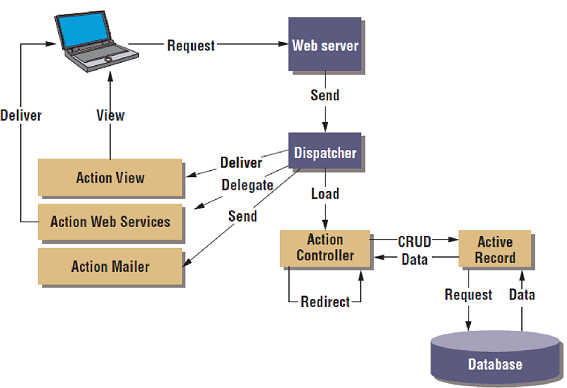
\includegraphics{Figs/frameworkRuby.png} % leia abaixo
	\label{figura:frameworkRuby}
\end{figure}
%Na seção seguinte será apresentada a maneira particular como o Rails realiza o mapeamento dos dados relacionais em objetos.
%Amparado nesta realidade, o presente trabalho, foi realizado utilizando a ferramenta Ruby on Rails. Nos próximos capítulos....
\section{Banco de Dados}

Para o desenvolvimento desse projeto, implementou-se um banco
de dados PostgreSQL, para armazenamento de informações sobre os usuários. A construção do Sistema de Gerenciamento de Banco de Dados do PostgreSQL foi iniciada em
1986. Os conceitos iniciais foram apresentados em \cite{stonebraker1986design}.  A primeira demonstração do sistema em operação foi realizada em 1987 e
o modelo de dados inicial apareceu em
\cite{stonebraker1988design}. 
Na seção seguinte serão apresentados os atores, requisitos funcionais e não funcionais, o diagrama de caso de uso e informações sobre o banco de dados utilizado.

\section{Requesitos do Sistema}
\subsection{Atores}
Os atores que poderão acessar o sistema são os seguintes:
 
 \textbf{Porteiro:} É o funcionário do IFRN responsável por realizar o cadastramento dos demais servidores ou alunos.
 
 \textbf{Administrador:} É o funcionário do setor de TI responsável pela administração da plataforma. Esse ator tem as permissões necessárias para gerenciar a plataforma, realizando atualizações e melhorias, se necessárias.
 \subsection{ Requisitos Funcionais}
 \label{Requisitos Funcionais}
 Na descrição desse tópico serão descritas as aplicações dos usuários definidos anteriormente.
As ações dos atores estão relacionadas aos requisitos estabelecidos pelo sistema \cite{SOMMERVILLE}, \cite{pressman2016engenharia}.\\\\\\1º Requisito Funcional\\
 \textbf{Cadastro de Usuários:} No software desenvolvido é utilizada a \texttt{gem} 'devise'  para cadastrar novos usuários.\\
 2º Requisito Funcional\\
 \textbf{Autenticação:}  A  \texttt{gem} 'devise' proporciona ao software a geração de uma tela de login onde o usuário
 informa suas habilitações obtendo acesso à plataforma de gerenciamento.
 3º Requisito Funcional\\
 \textbf{Redefinição de Senha:} A  \texttt{gem} 'devise' prepara a página de cadastramento de maneira que possa  enviar um link para o e-
 -mail do usuário para redefinição de senha, caso seja solicitada.\\
  4º Requisito Funcional\\
 \textbf{Cadastramento do estacionamento:}
 A  \texttt{gem} 'Admin' permite a geração de modelos sem a necessidade da criação de \textit{Controller} ou rotas. Dessa maneira, gerou-se os demais modelos, a saber, modelos para o cadastramento de: \textbf{veículo},
  %6º Requisito Funcional\\
 \textbf{tipo de vaga} e
  %7º Requisito Funcional\\
 \textbf{funcionário}.\\
 5º Requisito Funcional\\
 \textbf{Edição dos cadastros:}  A  \texttt{gem} 'Admin' prepara automaticamente a possibilidade de edição dos cadastros realizados. Nesse caso é possível atualizar, remover e exportar.
 
 \subsection{Requisitos Não-Funcionais}
 Define-se requisitos não-funcionais como aqueles que não possuem relacionamento direto com
 as atividades do software. Porém, são limitações dos serviços oferecidos pelo
 software \cite{rezende2006engenharia}.\\
 1º Requisito Não-Funcional\\
 \textbf{Incompatibilidade com dispositivos móveis:}
 O software não é compatível com dispositivos móveis.\\
 2º Requisito Não-Funcional\\
 \textbf{Acessos Simultâneos:}
 O banco de dados \texttt{postgresql} não possui limitação. No entanto, para proteção de acessos simultâneos, configurou-se um limite, restrito a uma faixa de IPs. Caso seja necessário uma maior capacidade, existe a possibilidade de modificação.
 
 \section{Diagrama de Casos de Uso}
 Levando-se em consideração as premissas anteriormente explicadas, pode-se modelar as funções do sistema proposto. Na Fig. \ref{figura:diagramaCasoUso_proj_vic} é apresentado o diagrama
 de casos de uso do sistema de gerenciamento de estacionamentos. Idealizou-se que o ator \textit{segurança} é o responsável pelo cadastramento, atualização e exclusão do ator \textit{Funcionário\_1}, que por sua vez, fornece seus dados pessoais e de seu veículo. 
 
 
 \begin{figure}[H]
 	\caption{Diagrama de Caso de Uso}
 	%\flushright
 	\centering % para centralizarmos a figura
 	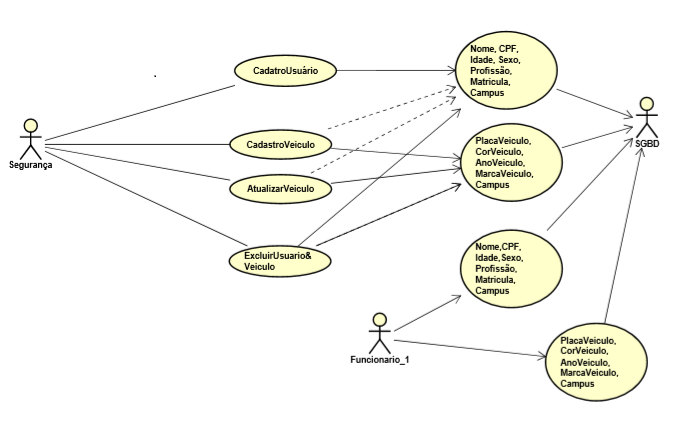
\includegraphics[scale=0.85]{Figs/diagramaCasoUso_proj_vic.png} % leia abaixo
 	\label{figura:diagramaCasoUso_proj_vic}
 \end{figure}



\section{Relacionamentos no RoR}
Comumente, sistemas que empregam orientação a objetos utilizam classes que retratam elementos reais do domínio de negócio. O sistema de gerenciamento de estacionamentos desenvolvido no presente trabalho possui as classes cujos modelos foram mencionados anteriormente (seção \ref{Requisitos Funcionais}). Essas classes de entidades em geral possuem relacionamentos que devem ser formalizados em código, isso quer dizer que essas classes precisam conter as informações de como devem atuar entre si. O framework Rails possui recursos para essa atividade. O tópico seguinte mostra alguns dos tipos mais impostantes de relacionamentos que podem existir entre as classes do modelo de uma aplicação.
\subsection{Tipos de relacionamentos}
Em \cite{relacionamentos2015} se lê:
\begin{citacao}
	
	Existem diversas formas de dois objetos se associarem entre si, os relacionamentos mais comuns entre classes são:
	\begin{itemize}
		
		\item Um para um. Onde um objeto pode estar associado a apenas outro objeto de um determinado tipo.
		\item Um para muitos. Neste caso um objeto poderá se associar com um ou vários objetos de outra classe.
		\item Muitos para muitos. Um objeto pode participar de vários relacionamentos com outros objetos de determinado tipo.
	\end{itemize}
\end{citacao}

A aplicação desses relacionamentos na estrutura Rails segue as seguintes formas: \texttt{belongs\_to} (pertence a), \texttt{has\_one} (tem um),\texttt{ has\_many} (tem muitos), \texttt{has\_and\_belongs\_to\_many} (tem e pertence a muitos), entre outras. Cada  método possui recursos que trazem efeitos ou modificações no banco de dados. No próximo tópico essas características serão discutidas.


\subsection{Associação \texttt{belongs\_to}}
Essa associação é geralmente denominada de \textit{um para um} e é utilizada para mostrar que um certo modelo \textit{pertence a} outro.

\subsection{Associação \texttt{has\_one}}
Essa ligação é do tipo \textit{um para um} e possui alguma semelhança com  \texttt{belongs\_to}. No entanto, preferivelmente, deve ser empregada em situações diferentes causando um efeito diferenciado. Tal associação é bidirecional a \texttt{belongs\_to}. A diferença mais significativa  é que não adiciona chave estrangeira ao modelo que a declara. 

\subsection{Associação \texttt{has\_many}}
Usa-se essa ligação entre modelos para indicar que o modelo em questão tem nenhum ou muitos elementos de outro modelo da aplicação. É denominada, frequentemente, de \textit{um para muitos}. Semelhante a \texttt{has\_one} ela não adiciona nenhuma coluna no modelo que a utiliza. Seu emprego deve ser em conjunto com \texttt{belong\_to} para indicar por meio de chave estrangeira com quem o objeto filho se relaciona. 

\subsection{Associação \texttt{has\_and\_belongs\_to\_many}}
Nessa opção é possível gerar uma ligação do tipo \textit{muitos para muitos} entre dois modelos da aplicação.
\section{Diagrama de Classes e seus Relacionamento}
Num diagrama de classes UML, as associações possibilitam a descrição de informações  nos extremos da linha que representa a ligação entre as classes. A Fig. \ref{figura:estacionamentoIfrn}
mostra os relacionamentos e os limites superiores (ou máximos) que representam a multiplicidade entre as classes.

\begin{figure}[h]
	\caption{Diagrama de Classes}
	%\flushright
	\centering % para centralizarmos a figura
	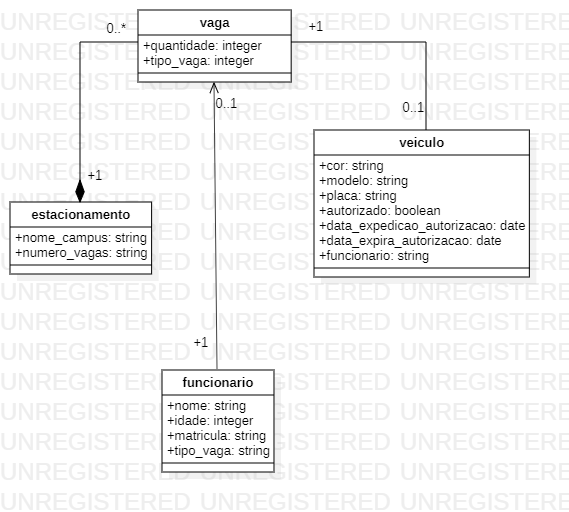
\includegraphics[scale=0.7]{Figs/estacionamentoIfrn_1.png} % leia abaixo
	\label{figura:estacionamentoIfrn}
\end{figure}


\section{Testes do Sistema}
\label{testesSoft}



Nessa seção serão apresentadas as telas da plataforma de gerenciamento de estacionamentos seguidas de descrições das funcionalidades.

Na tela mostrada na Fig. \ref{figura:signUp_projetoTCC} o usuário insere as credenciais para ser admitido no
sistema. A Fig. \ref{figura:signedUpSuccessfully} mostra a tela de confirmação de cadastramento do usuário. Ele deve cadastrar o estacionamento, indicando o campus, o funcionário, que possui direito a um tipo de vaga no estacionamento e seu veículo. As telas com esses direcionamentos são exibidas na sequência.


%Atualmente trabalha-se na definição dos relacionamentos entre os modelos. Foi possível, até o momento, realizar o cadastramento de estacionamentos, conforme mostra a Fig. \ref{figura:cadastroEstacionamentoCreated}.






\begin{figure}[h]
	\caption{Tela de Cadastramento do Usuário.}
	
	\centering % para centralizarmos a figura
	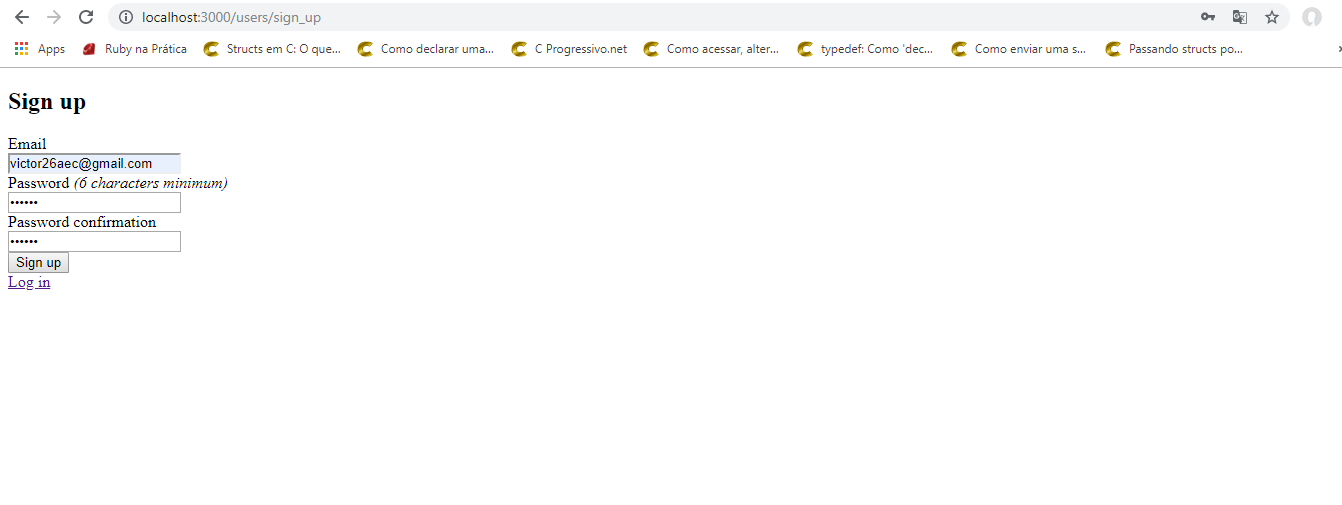
\includegraphics[scale=0.45]{Figs/signUp_projetoTCC.png} % leia abaixo
	\label{figura:signUp_projetoTCC}
\end{figure}

\begin{figure}[h]
	\caption{Tela de Confirmação de Cadastramento do Usuário.}
	
	\centering % para centralizarmos a figura
	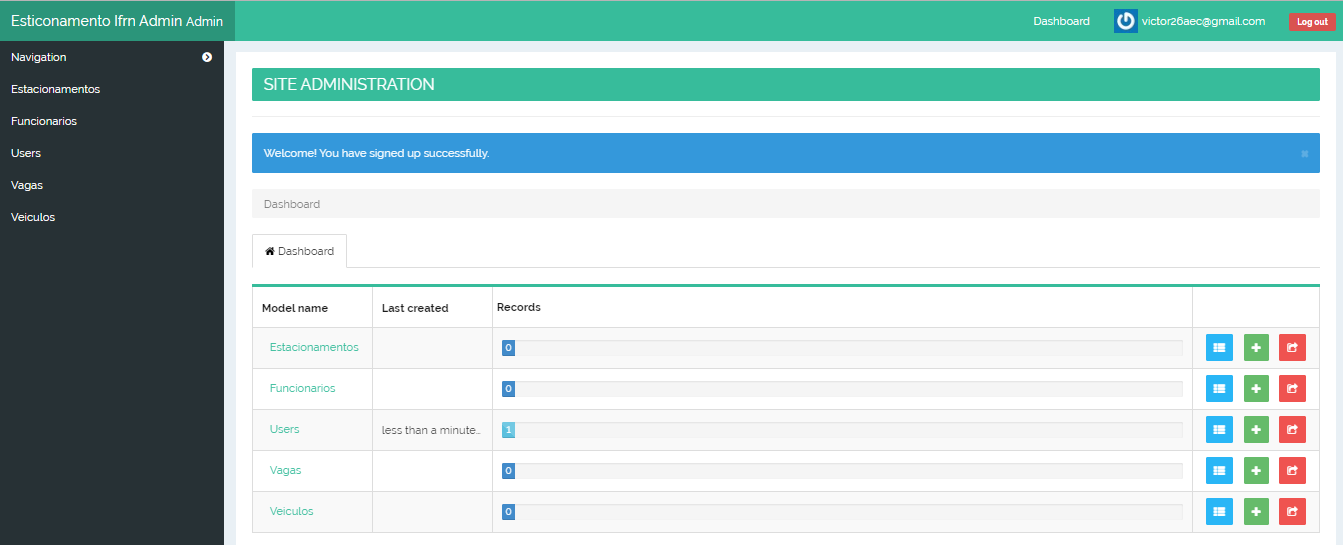
\includegraphics[scale=0.45]{Figs/signedUpSuccessfully.png} % leia abaixo
	\label{figura:signedUpSuccessfully}
\end{figure}

\begin{figure}[h]
	\caption{Tela de Confirmação de Cadastramento de Funcionário.}
	
	\centering % para centralizarmos a figura
	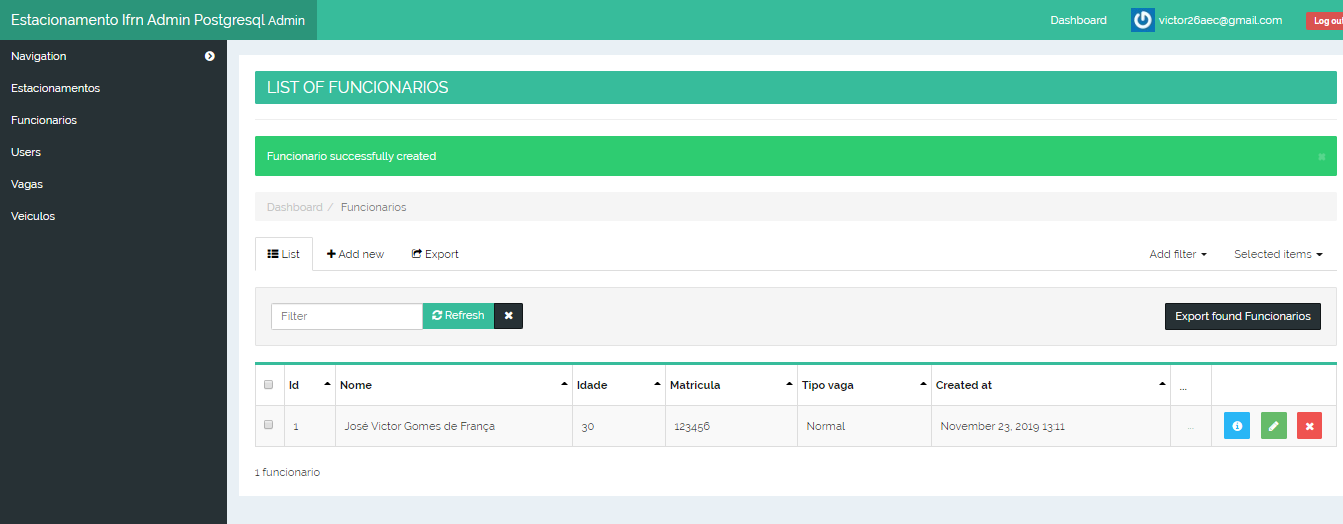
\includegraphics[scale=0.45]{Figs/funcionarioSuccessfullyCreated.png} % leia abaixo
	\label{figura:funcionarioSuccessfullyCreated}
\end{figure}

\begin{figure}[h]
	\caption{Tela de Confirmação de Cadastramento de Estacionamento.}
	
	\centering % para centralizarmos a figura
	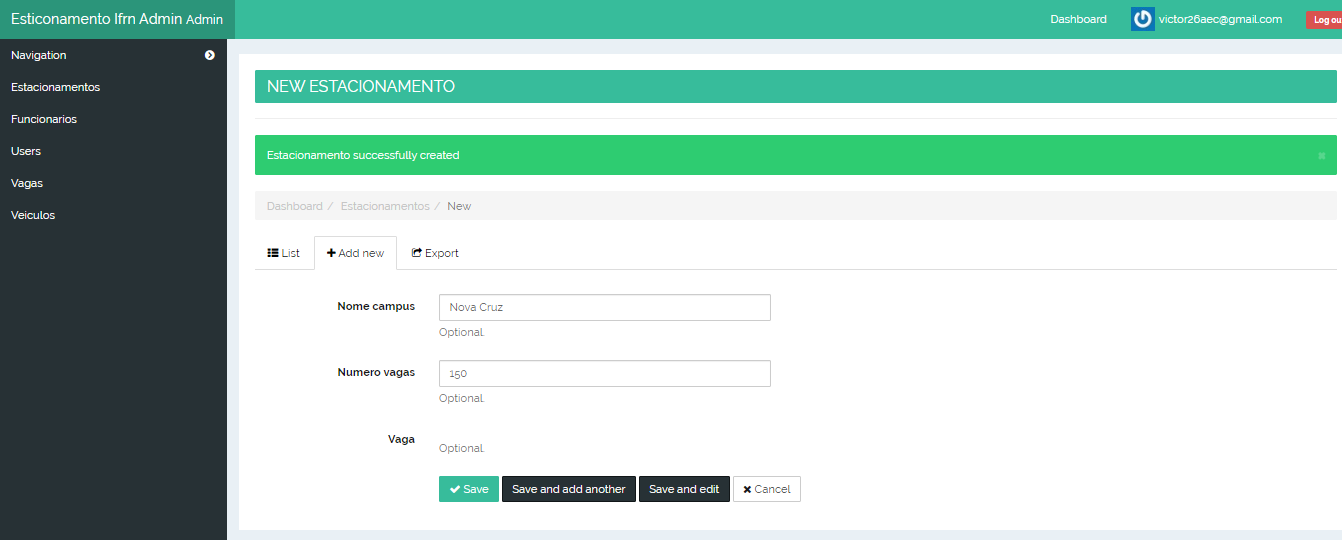
\includegraphics[scale=0.45]{Figs/cadastroEstacionamentoCreated.png} % leia abaixo
	\label{figura:cadastroEstacionamentoCreated}
\end{figure}



 
 \begin{figure}[h]
 	\caption{Tela de Confirmação de Cadastramento de Vaga.}
 	
 	\centering % para centralizarmos a figura
 	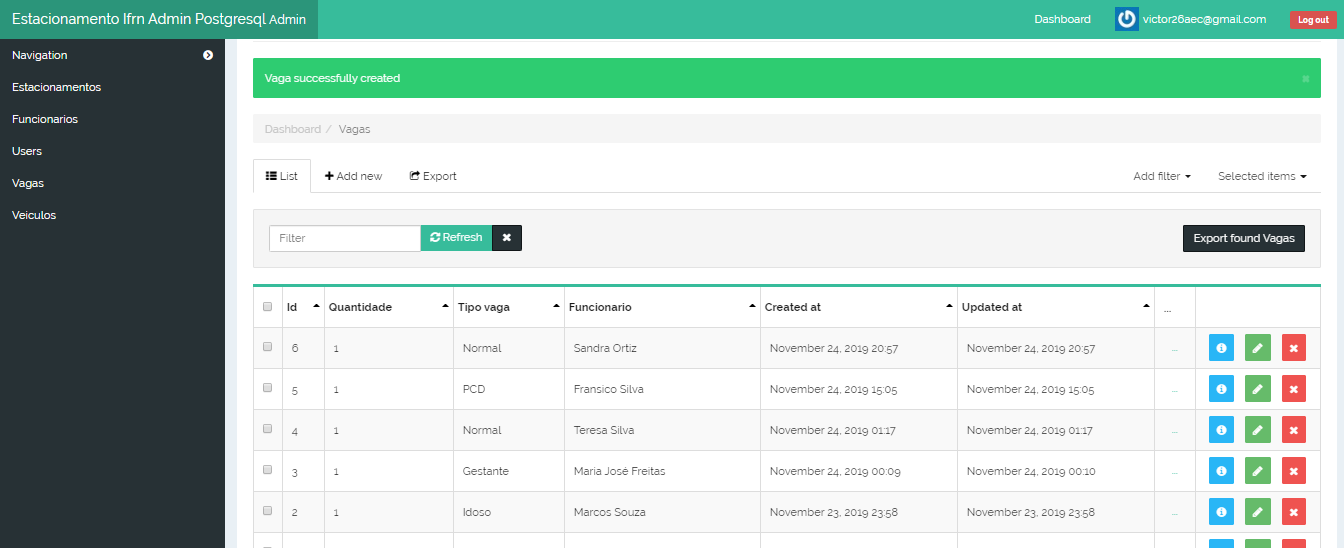
\includegraphics[scale=0.45]{Figs/vagaSuccessfullyCreated.png} % leia abaixo
 	\label{figura:vagaSuccessfullyCreated}
 \end{figure}

\begin{figure}[h]
	\caption{Tela de Confirmação de Cadastramento de Veículo.}
	
	\centering % para centralizarmos a figura
	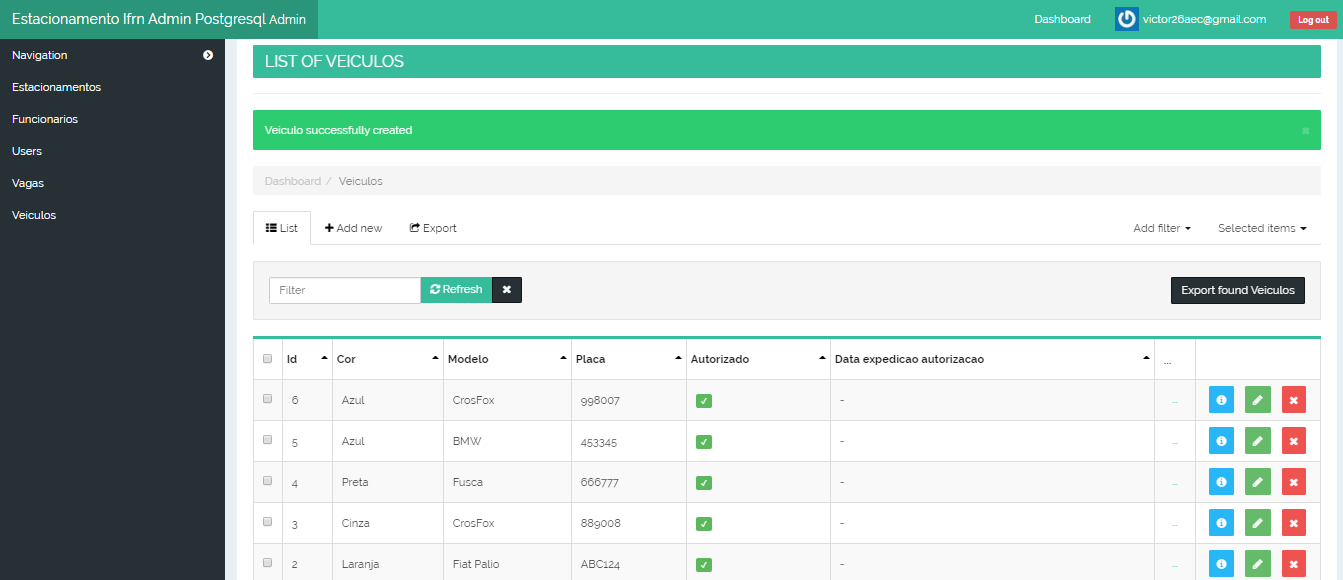
\includegraphics[scale=0.45]{Figs/cadastroVeiculoCreated.png} % leia abaixo
	\label{figura:cadastroVeiculoCreated}
\end{figure}
%\lipsum[34-36]
\chapter{Materiais e Métodos}\label{cap:ferramentas}

\lipsum[43-45]

\section{Considerações Finais}

\lipsum[23]


% PARTE
\part{Proposta}
\chapter{Sistema Proposto}\label{cap:proposta}

Esse trabalho propõe um sistema de... 


\section{Primeira Parte do Sistema Proposto}

\lipsum[67]

\section{Considerações Finais}

\lipsum[68]


% PARTE
\part{Parte Final}
\chapter{Resultados e Discussão}\label{cap:resultados}

\lipsum[73]

\section{Base de Dados}

\lipsum[72]

\section{Considerações Finais}

\lipsum[74]
\chapter*{Conclusões e Trabalhos Futuros}\label{cap:conclusao}
\addcontentsline{toc}{chapter}{Conclusão e Trabalhos Futuros}

\lipsum[81]

\section*{Conclusões}

\lipsum[82-84]

\section*{Trabalhos Futuros}

\lipsum[85] 

% ----------------------------------------------------------
% ELEMENTOS PÓS-TEXTUAIS (Referências, Glossário, Apêndices)
% ----------------------------------------------------------
\postextual

% Referências bibliográficas
\bibliography{bibliografia}

% Glossário (Consulte o manual)
%\glossary

% Apêndices
% ----------------------------------------------------------
% Apêndices
% ----------------------------------------------------------

% ---
% Inicia os apêndices
% ---
\begin{apendicesenv}

% Imprime uma página indicando o início dos apêndices
\partapendices

% ----------------------------------------------------------
\chapter{Primeiro Apêncice}
% ----------------------------------------------------------

\lipsum[50] % Texto qualquer. REMOVER!!

% ----------------------------------------------------------
\chapter{Perceba que o texto do título desse segundo apêndice é bem grande}
% ----------------------------------------------------------
\lipsum[51-53] % Texto qualquer. REMOVER!!

\end{apendicesenv}
% ---

% Anexos
% ----------------------------------------------------------
% Apêndices
% ----------------------------------------------------------

% ---
% Inicia os anexos
% ---
\begin{anexosenv}

% Imprime uma página indicando o início dos anexos
\partanexos

% ---
\chapter{Nome do Primeiro Anexo}
% ---
\lipsum[30] % Texto qualquer. REMOVER!!

% ---
\chapter{Nome de Outro Anexo}
% ---

\lipsum[32] % Texto qualquer. REMOVER!!

\end{anexosenv}

% Índice remissivo (Consultar manual)
%\phantompart
%\printindex

\end{document}
